\paragraph{La classe Dispatcher}


\begin{minipage}
    {\linewidth}
    \centering
    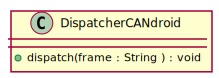
\includegraphics[width=0.50\linewidth]{../schemas/Conception_detaillee/classe_dispatcher_candroid.pdf}
    \captionof{figure}{Diagramme de classe de DispatcherCANdroid}
\end{minipage}
\subparagraph{Philosophie de conception \newline} 

\medspace


La classe DispatcherCANdroid a pour objectif de faciliter la communication. Elle joue le rôle d'intermédiaire entre la classe CommunicationCANdroid et la classe LogManager. Elle permet une communication centralisée et efficace dans l'application {\nomApplication}. 

\subparagraph{Description structurelle \newline}


\medspace

\textbf{Attributs :}

N.A.

\textbf{Services offerts :}

\begin{itemize}
    \item \textbf{dispatch(frame : String) : void} --- Opération qui permet l'envoi de la trame vers logManager pour ensuite l'afficher. 
\end{itemize}